\documentclass{beamer}
\usepackage[utf8]{inputenc}
\usepackage[frenchb]{babel}
\usepackage[T1]{fontenc}
\usepackage{graphics}
\usepackage{framed}
\usepackage{graphicx}
\usepackage{subcaption}
\usepackage{grffile}
\usepackage{longtable}
\usepackage{wrapfig}
\usepackage{rotating}
\usepackage[normalem]{ulem}
\usepackage{amsmath}
\usepackage{textcomp}
\usepackage{amssymb}
\usepackage{capt-of}
\usetheme{Madrid}

\title[Support pour Verificarlo]{Support de MPI et de la vectorisation dans Verificarlo}
\subtitle{Master Calcul Haute Performance et Simulation}

\author[Hery, Nicolas, Ali]{Hery ANDRIANANTENAINA \\ Nicolas BOUTON \\ Ali LAKBAL}

\institute[]{\textbf{Encadrant:} Eric PETIT}

\date{Année 2020-2021}

\begin{document}

\maketitle

% Nicolas
\begin{frame}{Verificarlo}

  \begin{block}{Compilateur s'appuyant sur}
    \begin{itemize}
    \item clang
    \item llvm
    \end{itemize}
  \end{block}

  \begin{block}{But}
    Intercepter les opérations flottantes afin de les analyser et les débogger
  \end{block}
  
\end{frame}

\begin{frame}{Rappel du backend VPREC}

  \begin{figure}
    \centering
    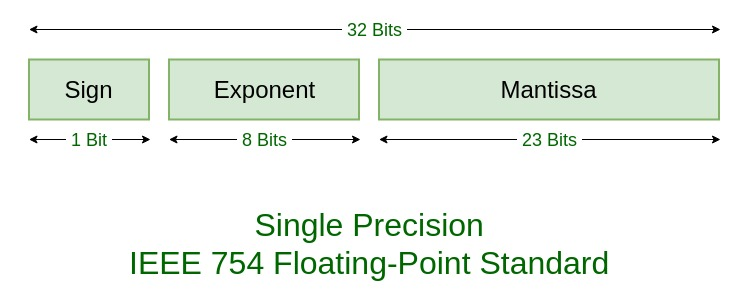
\includegraphics[width=200px]{../ressources/ieee754_floating-point_single_precision.jpg}
    \caption{\label{fig:ieee754_single_precision}Représentation d'un nombre flottant simple précision}
  \end{figure}

  \begin{block}{Cas spéciaux}
    \begin{itemize}
    \item NaN (Not a Number - Pas un Nombre)
    \item nombres infinis
    \item nombres dénormaux
    \end{itemize}
  \end{block}

\end{frame}

\begin{frame}{Changements aux niveaux du backend VPREC}

  \begin{figure}
    \centering
    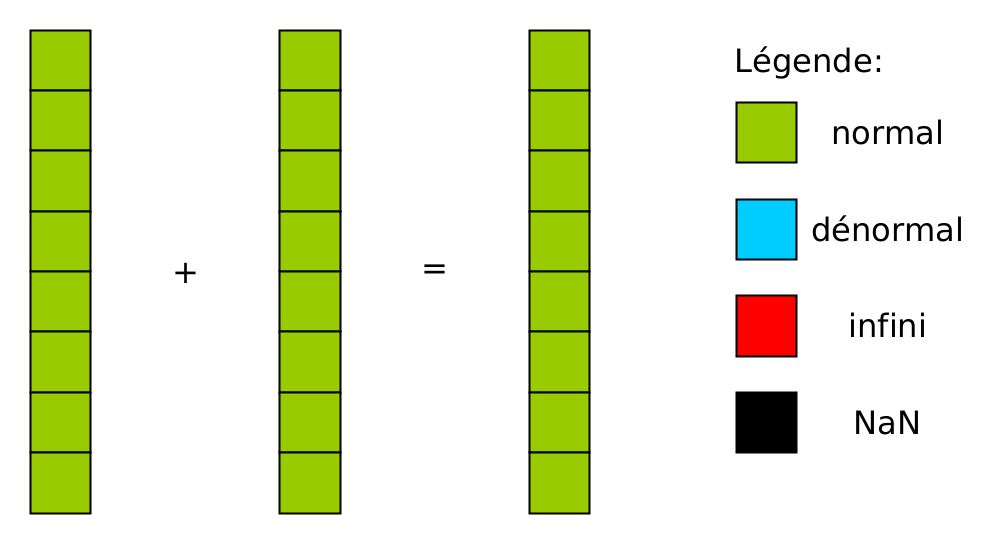
\includegraphics[width=300px]{../ressources/op_normal}
    \caption{\label{fig:ieee_simple_precision}Addition de 2 vecteurs de 8
      flottants simple précision générant un vecteur contenant que des nombres normaux}
  \end{figure}

\end{frame}

\begin{frame}{Changements aux niveaux du backend VPREC}

  \begin{figure}
    \centering
    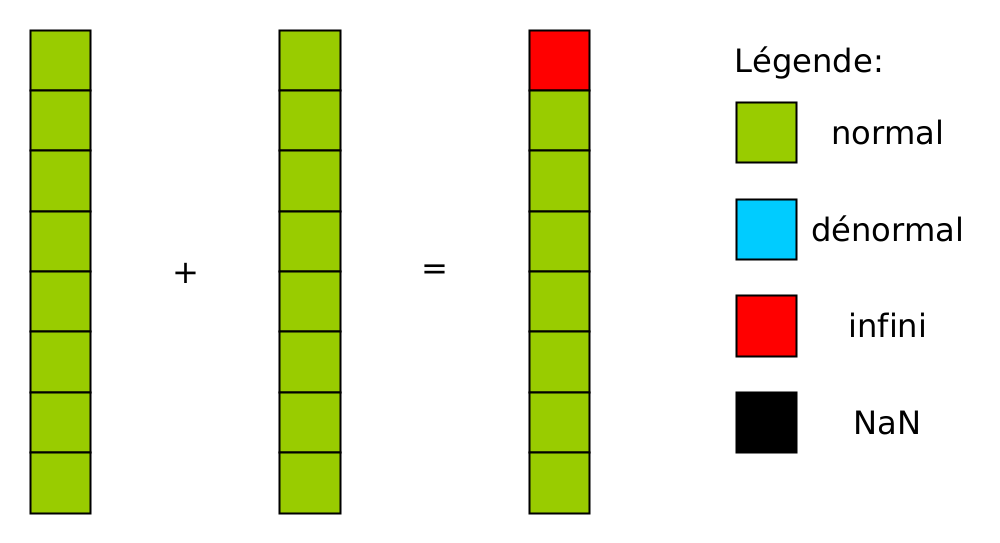
\includegraphics[width=300px]{../ressources/op_infini}
    \caption{\label{fig:ieee_simple_precision}Addition de 2 vecteurs de 8
      flottants simple précision générant un vecteur contenant un élément infini}
  \end{figure}

\end{frame}

% Ali
\begin{frame}{Benchmark}
  
  \begin{block}{But}
    \begin{itemize}
    \item Tester les performances de l'implementation vectorielle par rapport à la version scalaire. 
    \end{itemize}
  \end{block}

  \begin{block}{Utilisation}
    \begin{itemize}
    \item Les backends IEEE et VPREC.
    \item Les jeux d'instructions SSE et AVX.
    \item Les flottants simple précision.
    \end{itemize}
  \end{block}

\end{frame}

\begin{frame}{Benchmark}

  \begin{block}{Micro-benchmark}
    \begin{itemize}
    \item Les boucles qui font les calculs que l'on mesure 
    \end{itemize}
  \end{block}

  \begin{block}{Métriques prises en compte}
    \begin{itemize}
      
    \item Le temps.
    \item L'écart type.
    \item L'accelération.
      
    \end{itemize}
  \end{block}
  
\end{frame}

\begin{frame}{Tests et résultats}

  \begin{block}{Tests}
    
    \begin{itemize}

    \item Plusieurs tentatives d'exécution.
    \item Machine virtuelle: supporte AVX.
    \item Linux natif: ne supporte pas AVX.
      
      
    \end{itemize}
  \end{block}

\end{frame}

\begin{frame}{VPREC : Ecart type sur une Machine Virtuelle}
  
  \centering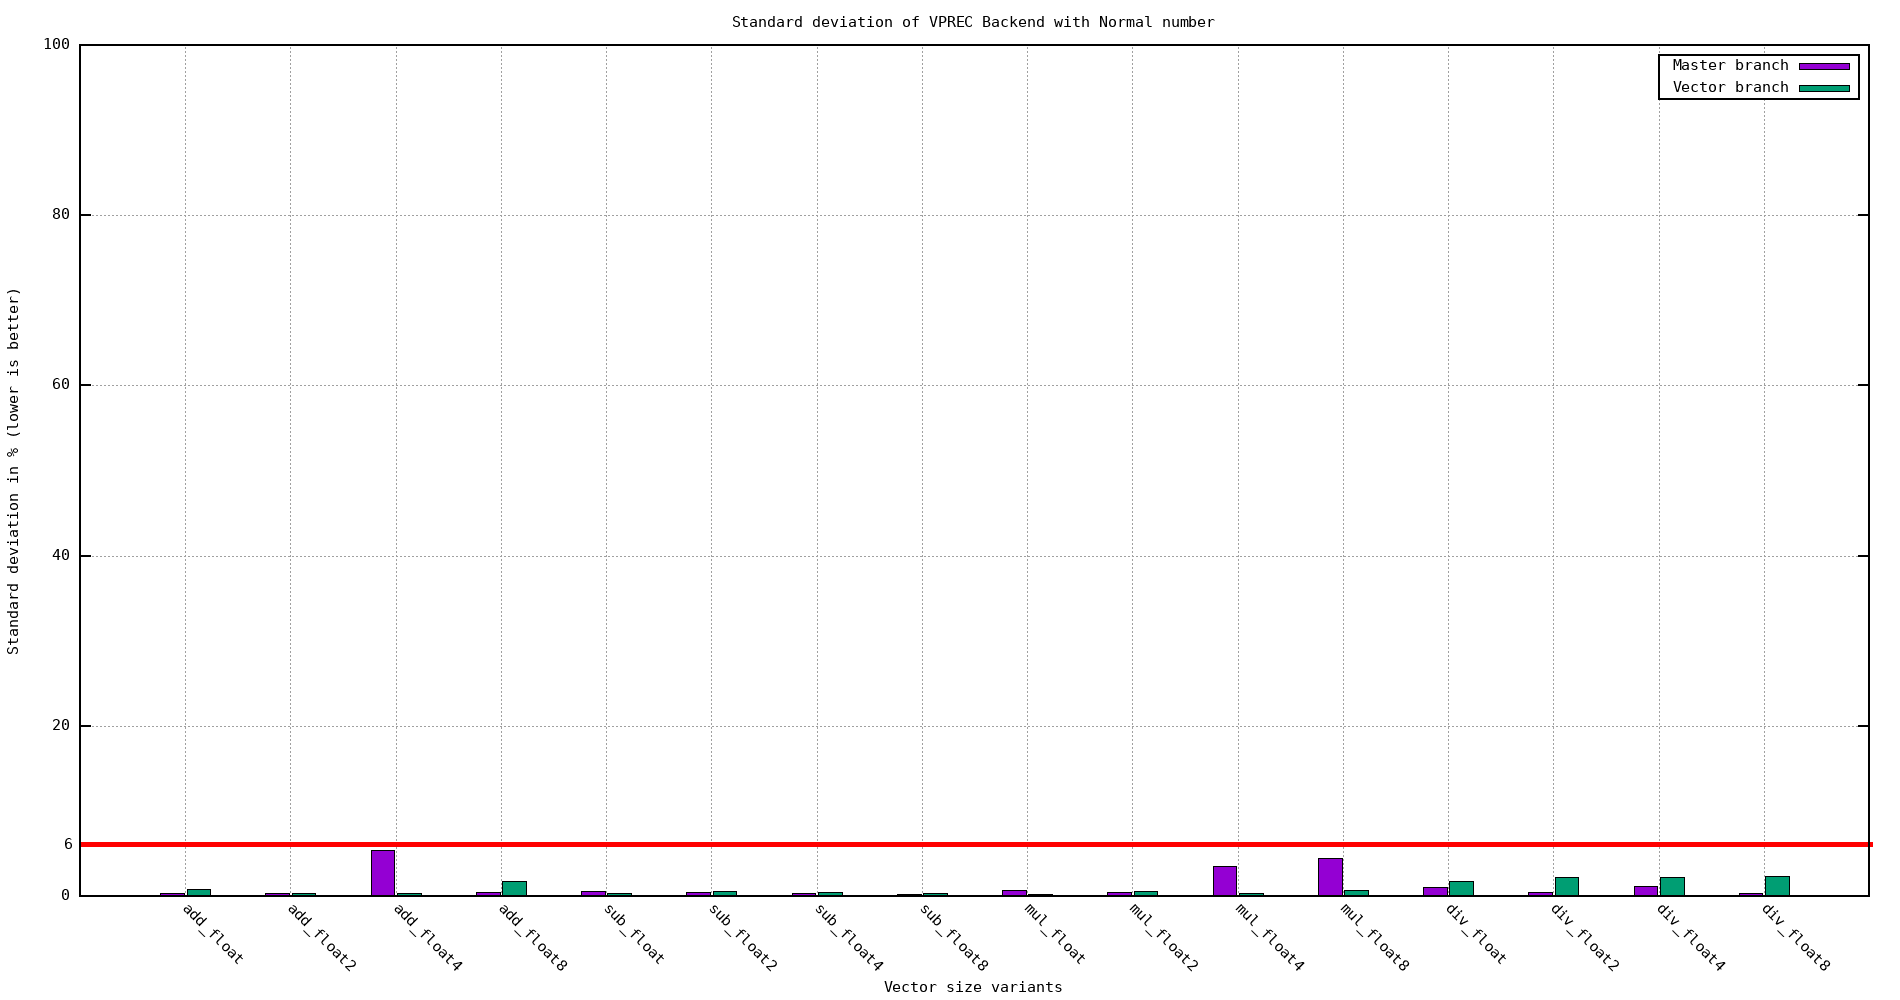
\includegraphics[width=200px]{../ressources/vm_vprec_normal_stddev.png}
  \centering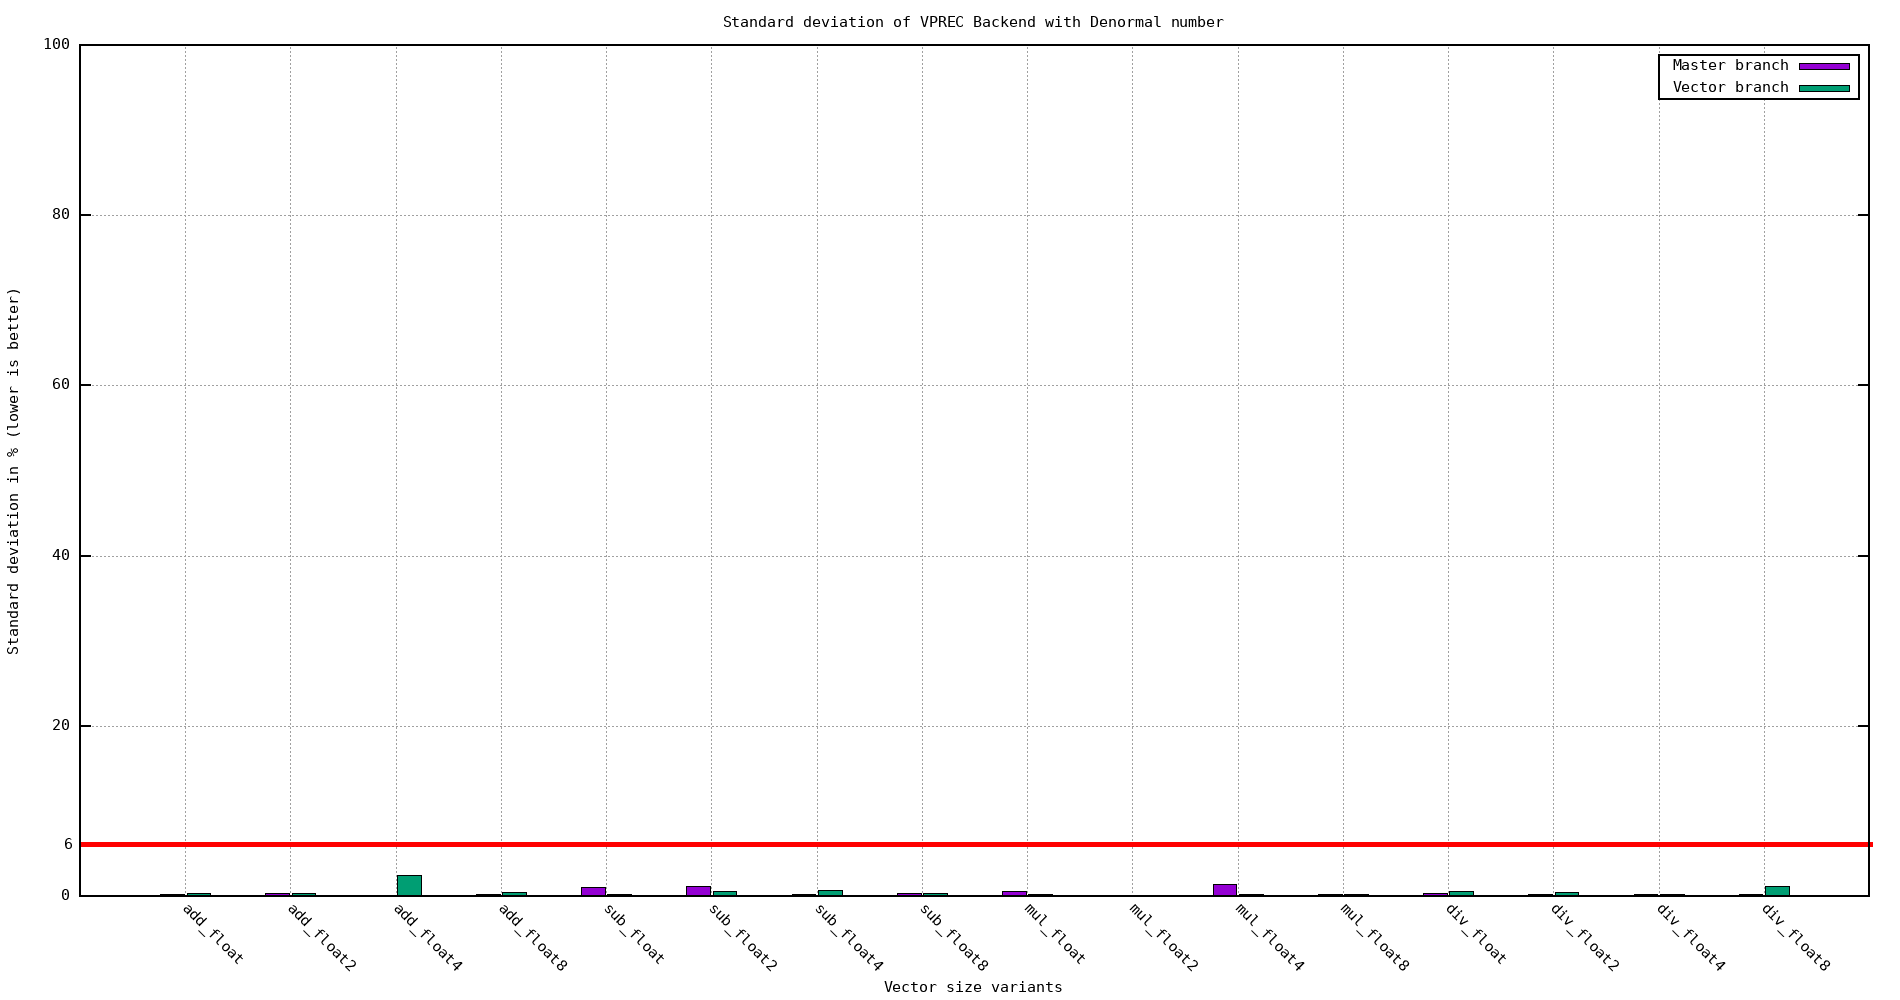
\includegraphics[width=200px]{../ressources/vm_vprec_denormal_stddev.png}
  
\end{frame}

\begin{frame}{VPREC: Ecart type sur un Linux natif}

  \centering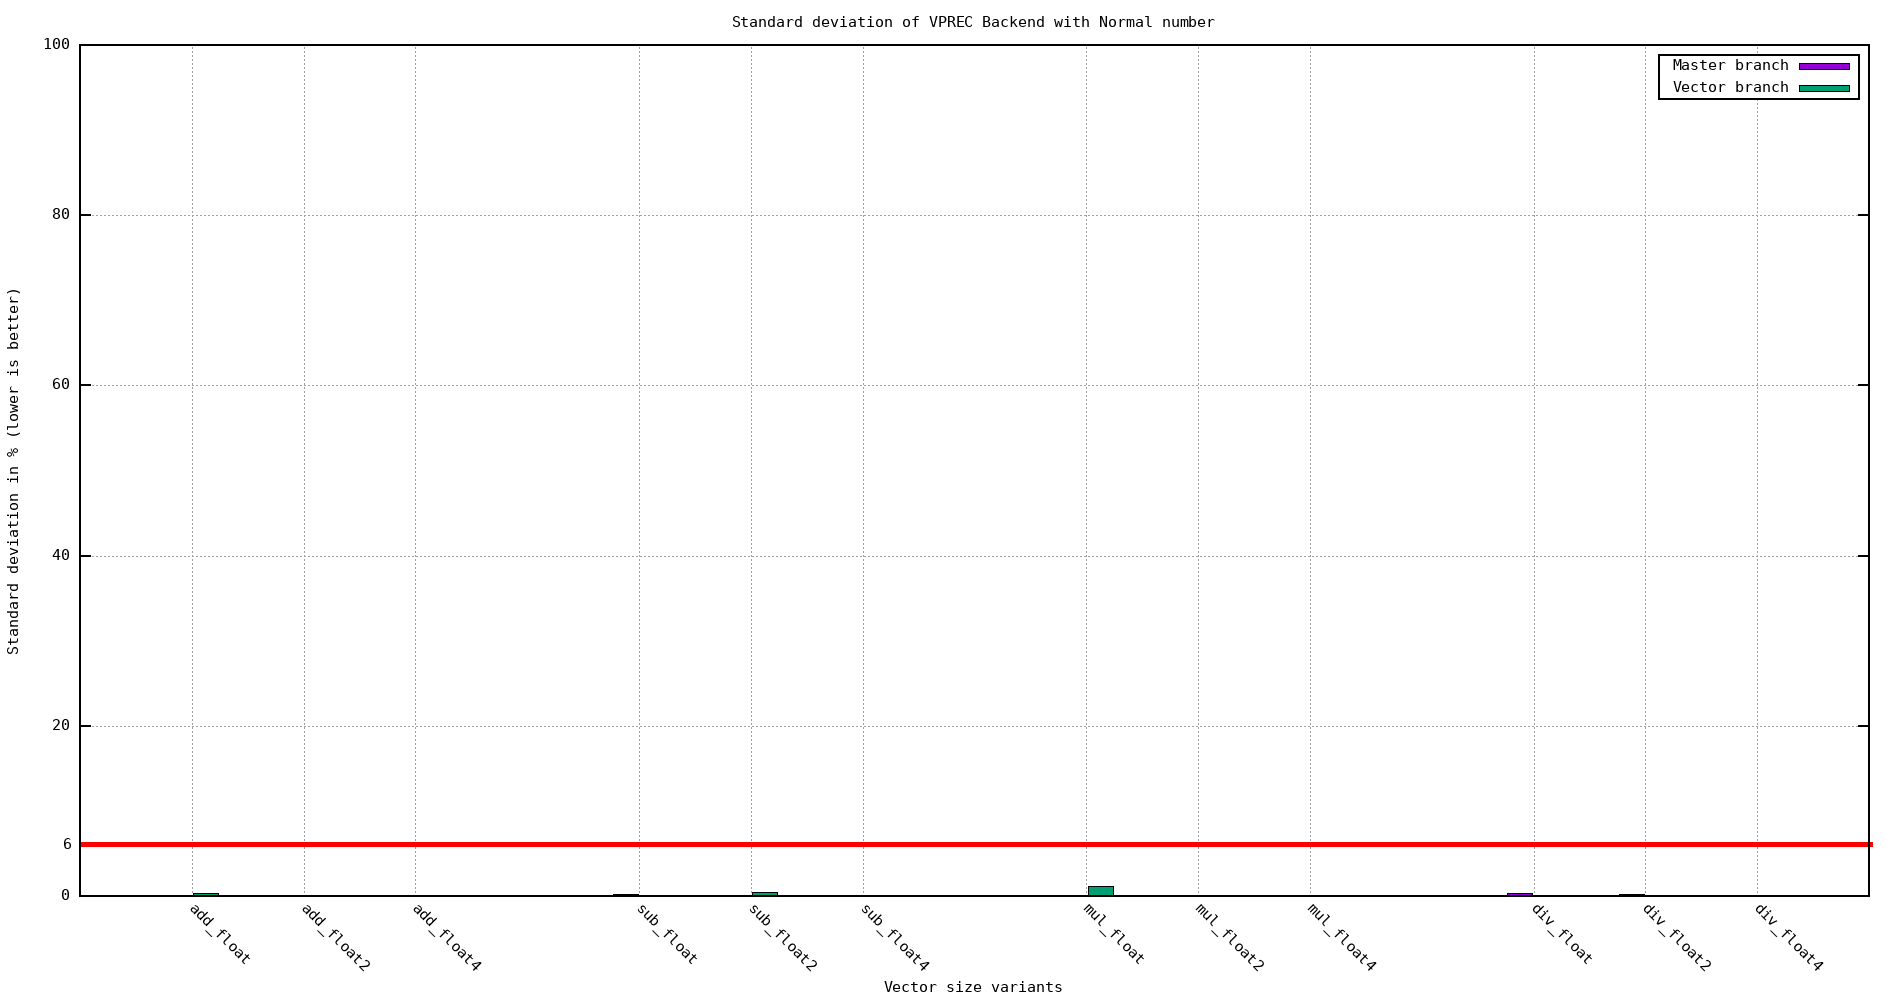
\includegraphics[width=220px]{../ressources/laptop_vprec_normal_stddev.png}
  \centering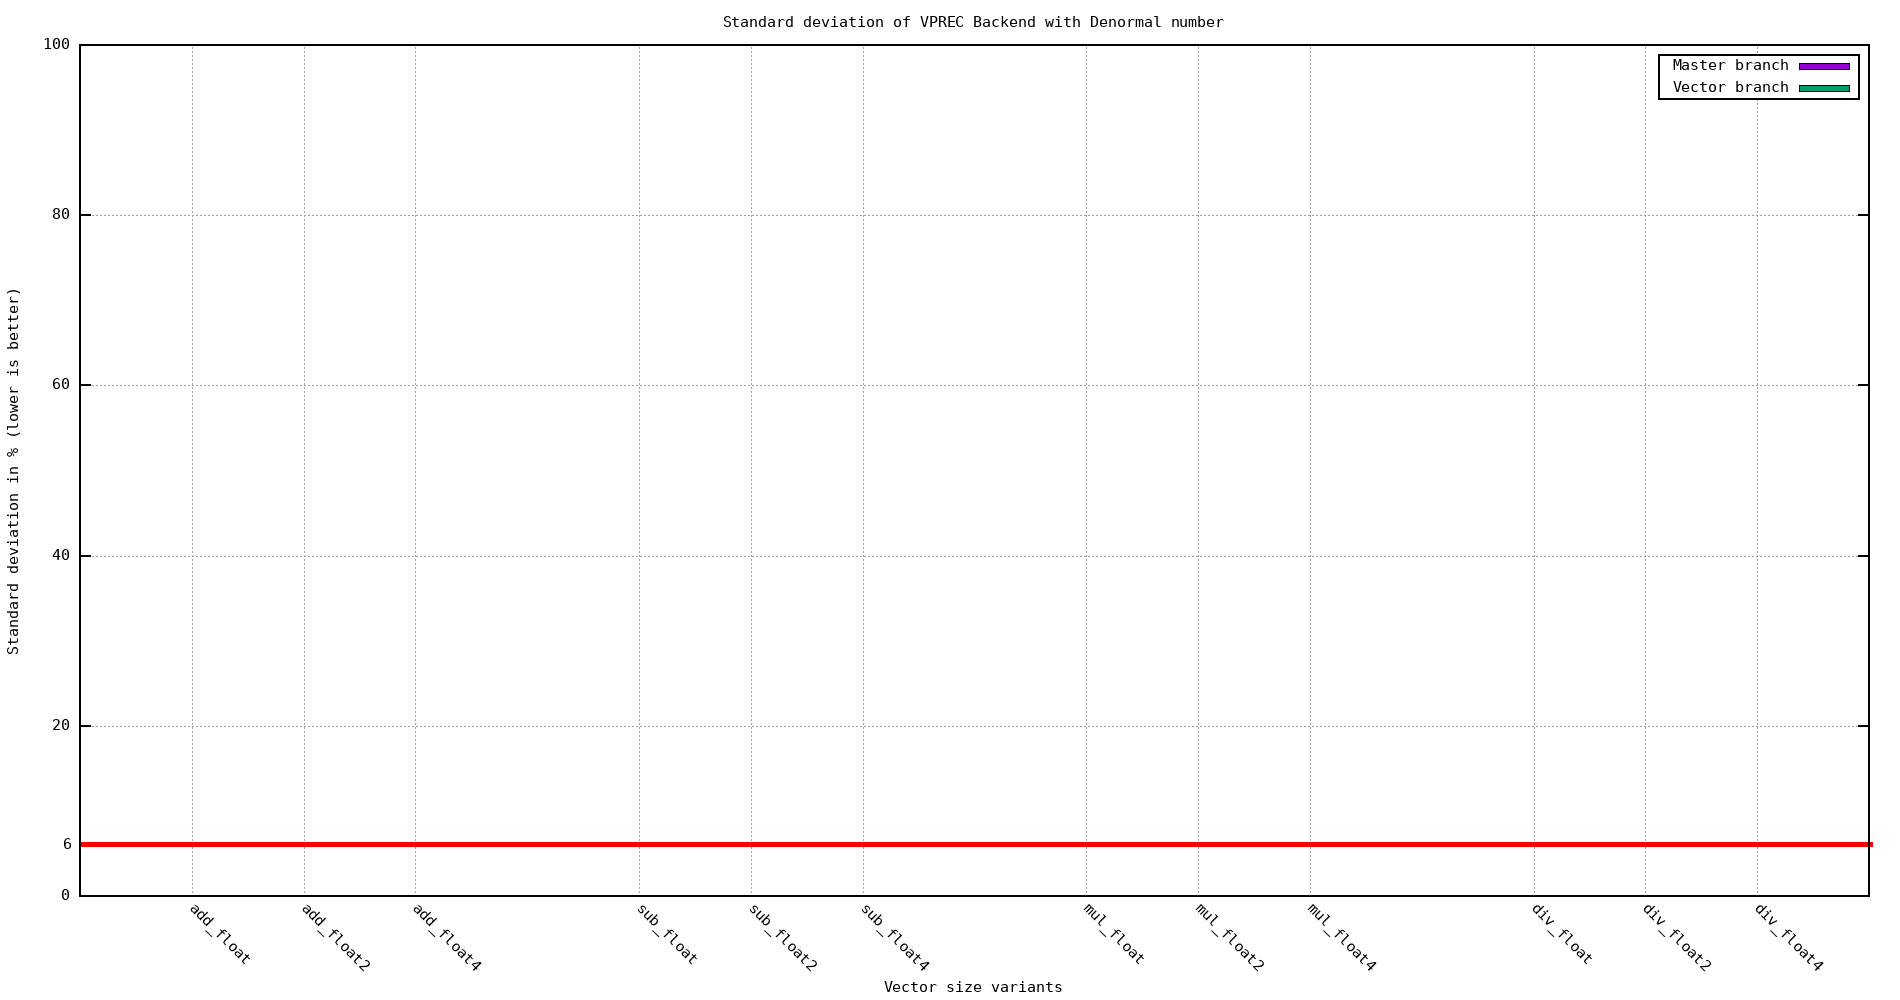
\includegraphics[width=220px]{../ressources/laptop_vprec_denormal_stddev.png}
  
\end{frame}

\begin{frame}{VPREC: Résultat d'accélération normaux/dénormaux}

  \centering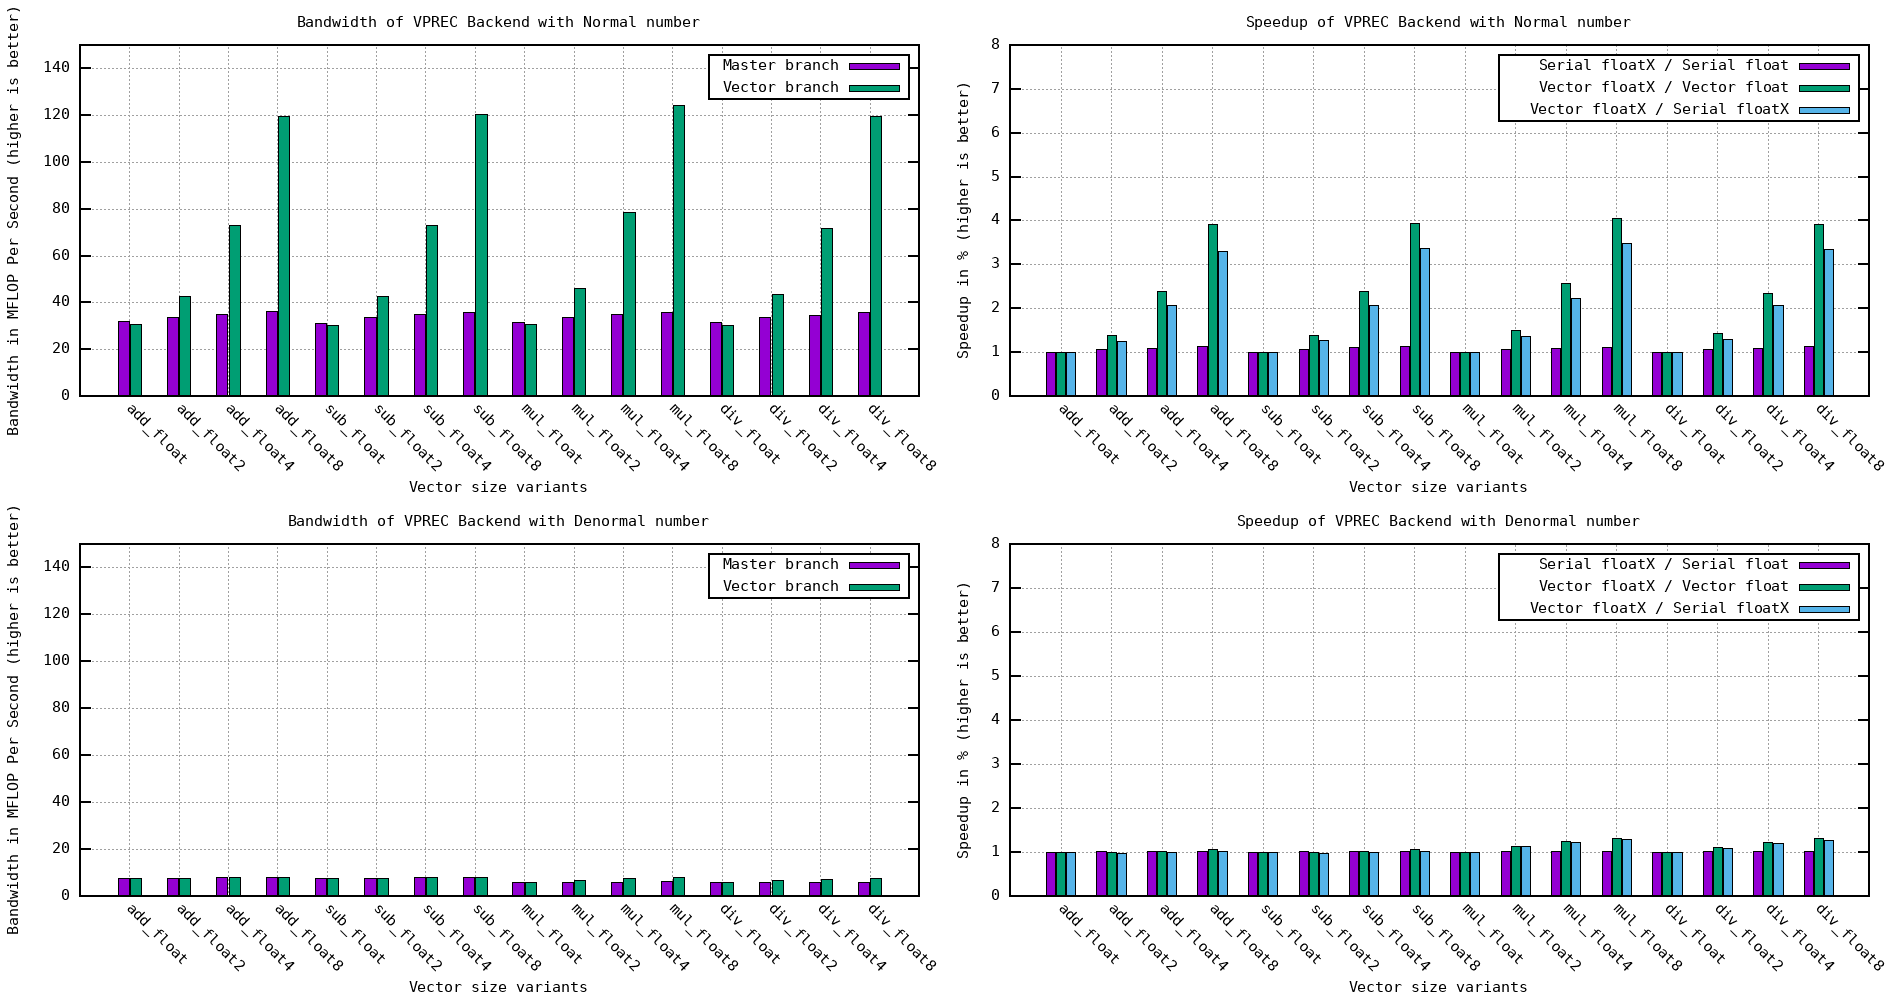
\includegraphics[width=340px]{../ressources/vm_vprec.png}
  
\end{frame}

\begin{frame}{IEEE: Ecart type}

  \centering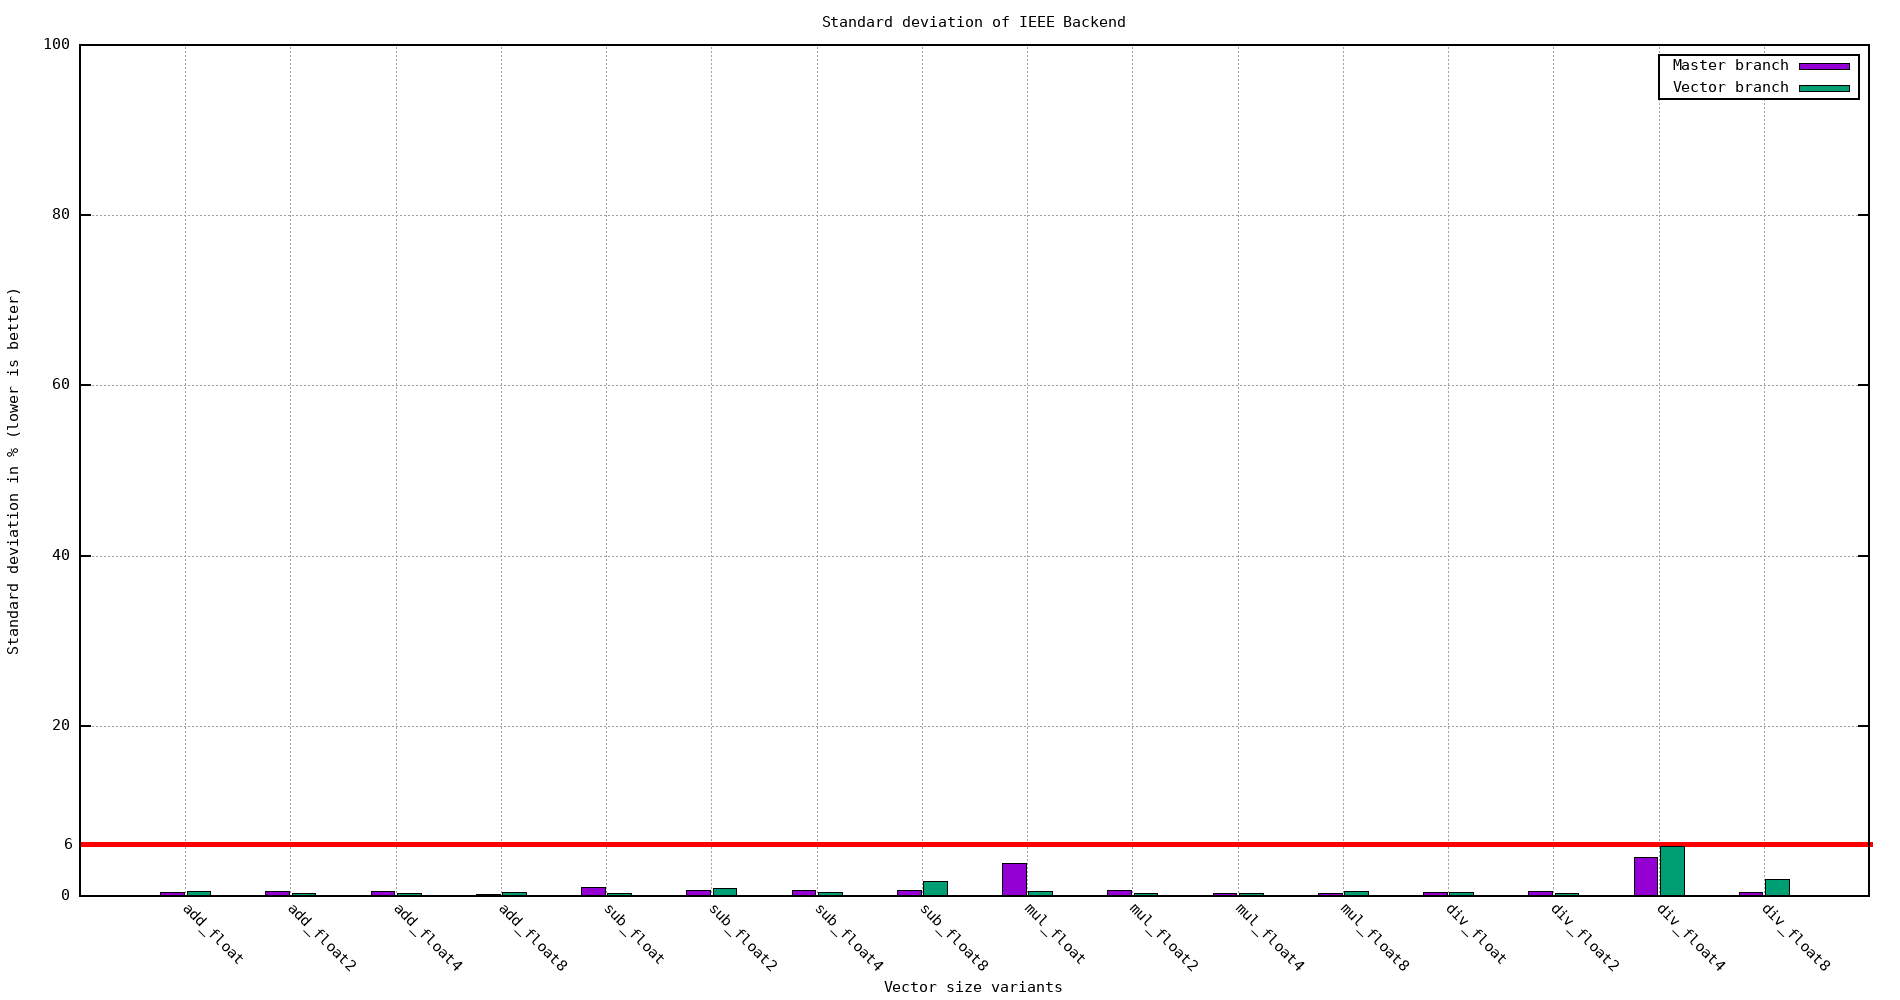
\includegraphics[width=300px]{../ressources/vm_ieee_stddev.png}
  
\end{frame}

\begin{frame}{IEEE: Accélération}

  \centering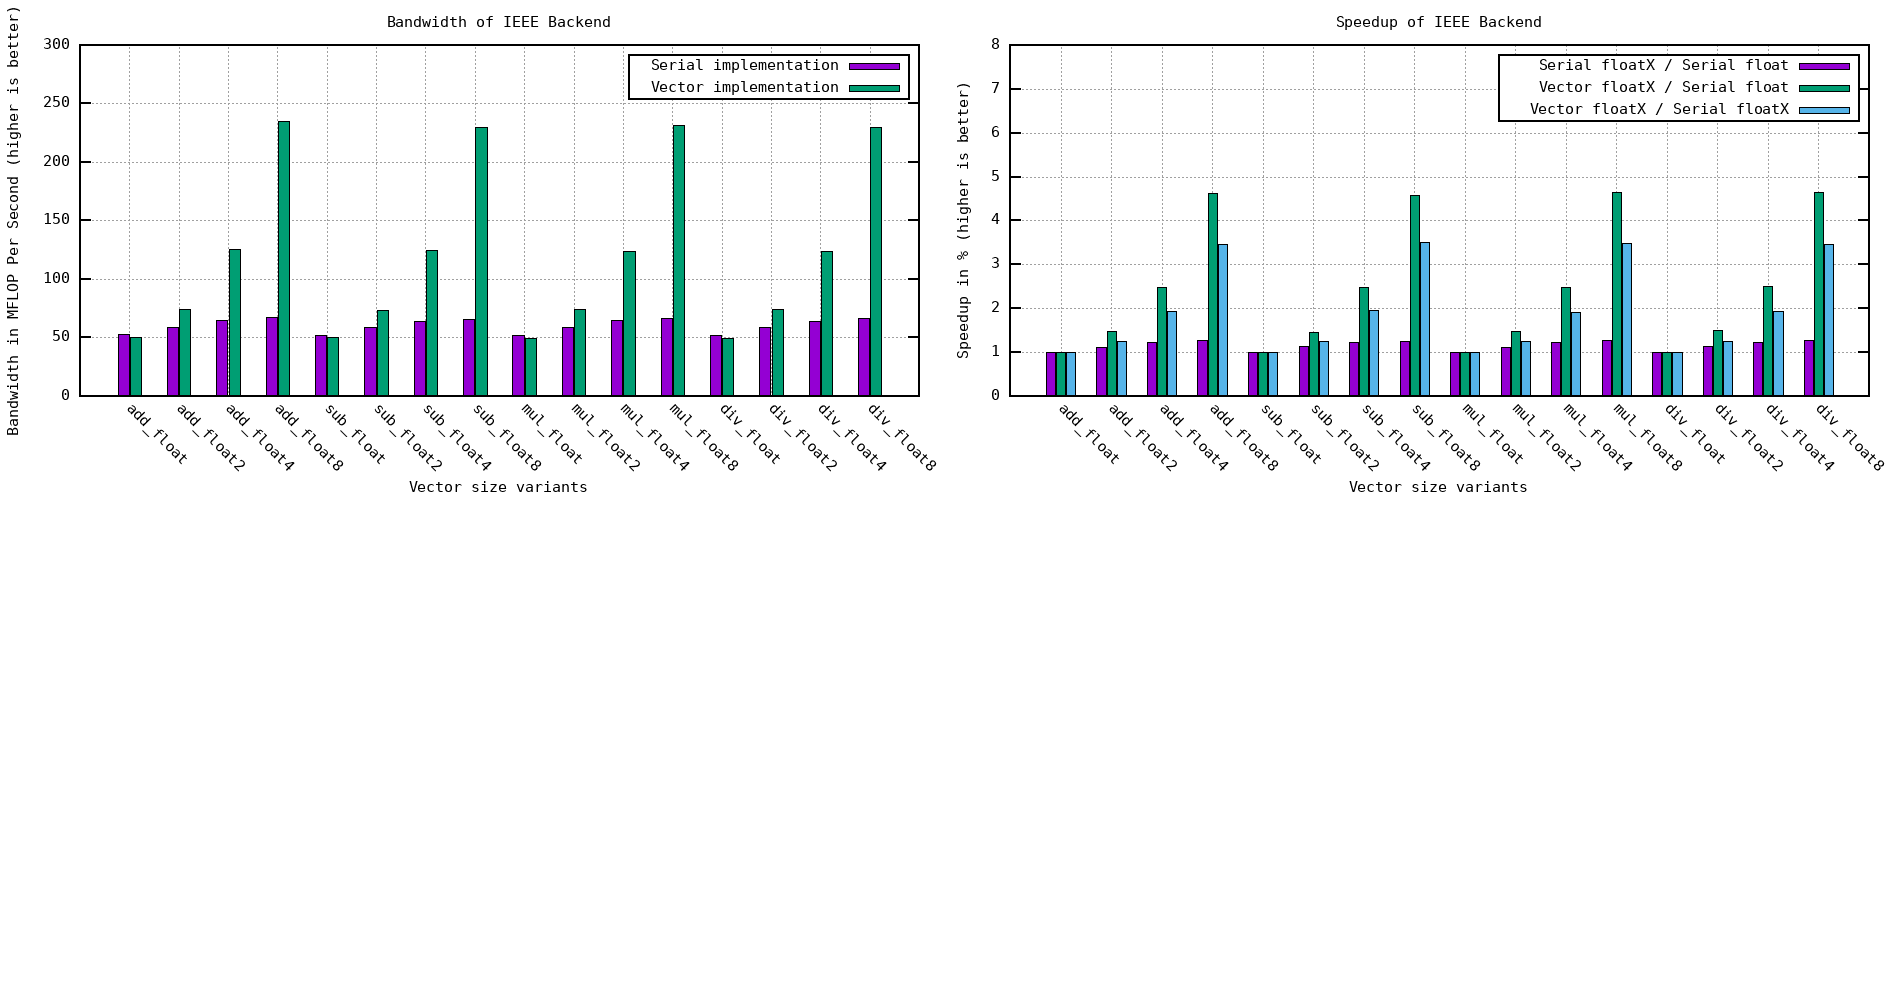
\includegraphics[width=350px]{../ressources/vm_ieee.png}
  
\end{frame}

% Hery
\begin{frame}{Support de la parallélisation}

  \begin{block}{Introduction}
    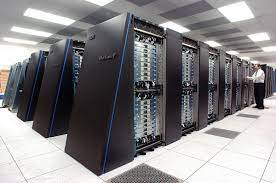
\includegraphics[width=0.6\linewidth]{../ressources/index.jpeg}
    source:fr.wikipedia.org
  \end{block}

\end{frame}

\begin{frame}{Différentes types de NAS Benchmarks Parallèle}

  \begin{block}{NPB1}
    \begin{itemize}
    \item Introduction des fonctions qui va facilité les parallélismes
    \item Vérification de la cohérence des résultats et de la performance
    \item Adaptation avec les systèmes à plusieurs coeurs.
    \end{itemize}
  \end{block}
  
  \begin{block}{NPB2}
    \begin{itemize}
    \item Modification des règles sur les analyses comparative
    \item Accès aux codes sources pour le grand public
    \item Version parallélisé avec MPI
    \end{itemize}
  \end{block}
  
  \begin{block}{NPB3}
    \begin{itemize}
    \item Version parallélisé avec openmp
    \item Version hybride ou "Multi-zone" 
    \end{itemize}
  \end{block}

\end{frame}

\begin{frame}{ Différentes types de benchmark}

  \begin{block}{Types}
    \begin{itemize}
    \item IS : "Integer Sort"
    \item EP : " Embarrassingly Parallel"
    \item CG : "Conjugate Gradient" 
    \item MG : "Multi-Grid"
    \item FT : "Fourier Transform"
    \item BT: "Block Tri-diagonal solver"
    \item SP: "Scalar Penta-diagonal solver"
    \item LU: "Lower-Upper Gauss-Seidel solver"
    \end{itemize}
  \end{block}
  
  \begin{block}{Classe}
    \begin{itemize}
    \item Classe S 
    \item  Classes A , B , C 
    \item Classes D , E , F
    \end{itemize}
  \end{block}
  
\end{frame}

\begin{frame}{ Résultat et discussion}

  \begin{block}{Compilation}
    CC=OMPI\_FC=verificarlo-f  mpif90
  \end{block}
  
  \begin{block}{Problème}
    Dimension sept pour les tableaux
  \end{block}
  
  \begin{block}{Solution}
    Ré-compilation
    \begin{itemize}
    \item CC=clang
    \item CXX=clang++
    \item FC=flang
    \end{itemize}
  \end{block}

\end{frame}

\begin{frame}{Résultat et discussion}

  \begin{block}{Test}
    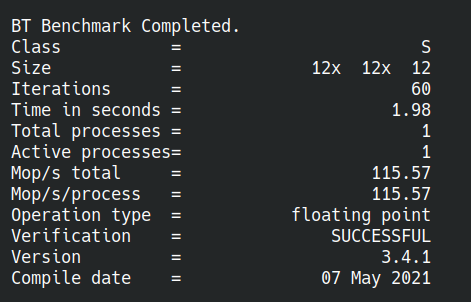
\includegraphics[width=0.6\linewidth]{../ressources/btcompleted.png}
  \end{block}

\end{frame}

\begin{frame}{Résultat et discussion}

  \begin{block}{Résultat vectorisation NPB-MPI FORTRAN}
    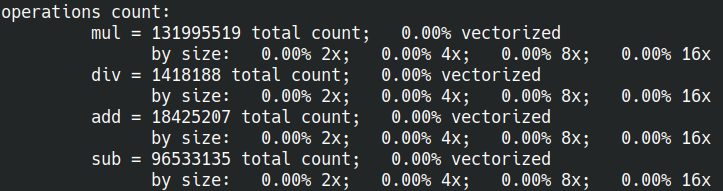
\includegraphics[width=0.6\linewidth]{../ressources/vect1.png}
  \end{block}
  
  \begin{block}{Résultat vectorisation NPB-OPENMP C}
    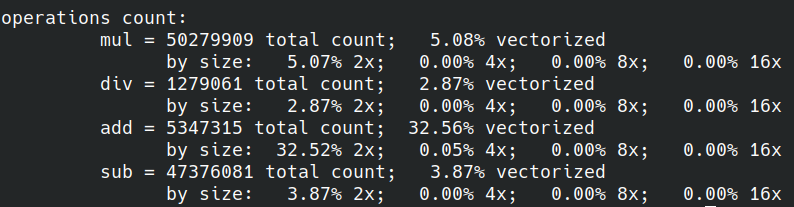
\includegraphics[width=0.6\linewidth]{../ressources/vcopenmp.png}
  \end{block}

\end{frame}

\begin{frame}{ Conclusion}

  \begin{block}{Test super-calculateur}
    \begin{itemize}
    \item Évaluation de la vectorisation sur le jeu d'instruction AVX512
    \item Faire des tests sur les problèmes de tailles standards ou les gros problèmes
    \end{itemize}
  \end{block}
  
  \begin{block}{Conclusion générale}
    \begin{itemize}
    \item Le module de Calcul Numérique sur la précision numérique qui est un des sujets principaux de verificarlo.
    \item Le module d’Architecture Parallèle et de Technique d’Optimisation Parallèle pour les mesures de performances et les benchmarks.
    \item Les modules traitant la parallélisation avec MPI et OpenMP comme Algorithme de Programmation Parallèle 
    \end{itemize}
  \end{block}
  
\end{frame}

\end{document}
